\documentclass{article}
\usepackage{fullpage}
\usepackage[normalem]{ulem}
\usepackage{amstext}
\usepackage{amsmath}
\usepackage{graphicx}
\newcommand{\var}[1]{\mathit{#1}}
\setlength{\parskip}{6pt}

\begin{document}

\noindent
University of Toronto\\
{\sc csc}321, Winter 2018\\[10pt]
{\LARGE\bf Assignment 4: Dominick Han 1001790591} \\[10pt]
\section*{Part 1: DCGAN}
The equation to calculate padding is:

$$O=\frac{(W-K+2P)}{S}+1$$

$$(O-1)S=W-K+2P$$

Giving that $W=2O, S=2, K=4$

$$2O-2=2O-4+2P$$

Therefore padding $P=1$



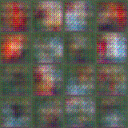
\includegraphics{samples_vanilla/sample-000200.png}

\includegraphics{samples_vanilla/sample-005600.png}

Here are images from iteration 200 and 5600.

We can see the first one (200 iterations) is almost not recognizable and very blurry, while the second one (5600 iterations) is less blurry and some what resembles emojis
\newpage

\section*{Part 2: CycleGAN}
\begin{enumerate}
\item
cyclegan (Iteration 600)


\includegraphics[scale=0.7]{samples_cyclegan/sample-000600-X-Y.png}

\includegraphics[scale=0.7]{samples_cyclegan/sample-000600-Y-X.png}

\item
cyclegan\_cycle (Iteration 600)


\includegraphics[scale=0.7]{samples_cyclegan_cycle/sample-000600-X-Y.png}

\includegraphics[scale=0.7]{samples_cyclegan_cycle/sample-000600-Y-X.png}

\item
cyclegan\_pretrained (Iteration 100)


\includegraphics[scale=0.7]{samples_cyclegan_pretrained/sample-000100-X-Y.png}

\includegraphics[scale=0.7]{samples_cyclegan_pretrained/sample-000100-Y-X.png}

\item
cyclegan\_cycle\_pretrained (Iteration 100)


\includegraphics[scale=0.7]{samples_cyclegan_cycle_pretrained/sample-000100-X-Y.png}

\includegraphics[scale=0.7]{samples_cyclegan_cycle_pretrained/sample-000100-Y-X.png}
\item
Explanations

At the first 600 iteration, we can already see that the model with cycle loss has more saturated color (more activated). It also has more details of the emoji compare to the first one

For the pretrained models, we can see that the one with cycle loss is more accurate (venezuela flag has irrelevant color in the model without the loss), and the model without cycle loss performed badly

Cycle consistency loss is a way to measure the loss when we transform the emojis from X to Y the back to X. For a perfect transformation, it should have 0 loss when we do this cycle transformation. Without optimizing on this cycle loss, the models might overfit/underfit and give out false output. (cycle consistency loss penalize false outputs)

\end{enumerate}
\end{document}